\documentclass[a4paper,11pt]{report}
\usepackage[margin=2cm]{geometry}
\usepackage{listings}
\usepackage{amsmath}
\usepackage{amssymb}
\usepackage{graphicx}
\usepackage{wrapfig}
\usepackage{algorithm}
\usepackage{algorithmicx}
\usepackage{algpseudocode}
\usepackage{tikz}

%%%%%%%%TIKZ SUDOKU%%%%%%%%%%
\newcounter{row}
\newcounter{col}
\newcounter{rowa}
\newcounter{cola}
\newcounter{rowb}
\newcounter{colb}

\newcommand\setrow[9]{
  \setcounter{col}{1}
  \foreach \n in {#1, #2, #3, #4, #5, #6, #7, #8, #9} {
    \edef\x{\value{col} - 0.5}
    \edef\y{9.5 - \value{row}}
    \node[anchor=center] at (\x, \y) {\n};
    \stepcounter{col}
  }
  \stepcounter{row}
}
\newcommand\setrowa[4]{
  \setcounter{cola}{1}
  \foreach \n in {#1, #2, #3, #4} {
    \edef\x{\value{cola} - 0.5}
    \edef\y{4.5 - \value{rowa}}
    \node[anchor=center] at (\x, \y) {\n};
    \stepcounter{cola}
  }
  \stepcounter{rowa}
}
%%%%%%%%%%%%%%%%%%%%%%%%

\author{E. Routledge}
\date{01 Nov 2022}
\title{Sudoku is Hard}


\begin{document}
\lstset{language=Python}
\maketitle
\begin{abstract}
sudoku overview
\end{abstract}
\tableofcontents
% ~~~~~~~~~~~~~~~~~~~~~~~~~~~~~~~~~~~~~~~~~~~~~~~~~~~~~~~~~~~~~~~~~~~~~~~~~~~~~~~~~~~~~~~~~~~~ %
\chapter{Introduction}
Sudoku is a simple logic game, in the standard $9 \times 9$ (or $3 \times 3 \times 3 \times 3$) one must complete the grid such
that every row, column and box contains the numbers 1 to 9, that is all, yet it is filled with mathematics. Through sudoku we
can explore the connections between various areas of maths: complexity theory, graph theory, group theory and information
theory.

	\section{History}
	
	\section{Defining Sudoku Notation}
	
\textbf{Def$^n$}: A valid sudoku puzzle is a function $ S: i,j \rightarrow x$ for values i,j $\in \{1,...,D^2\}$ and $x \in
\{0,...,D^2\}$ satisfying the following:
\begin{itemize}
	\item{for all $a,b,c$  $\in \{1,...,D^2\}$ with $S(a,b)\neq$ 0 and $S(a,c)\neq$ 0, then $ S(a,b)\neq$ S(a,c) }
	\item{for all $a,b,c$  $\in \{1,...,D^2\}$ with $S(a,b)\neq$ 0 and$ S(c,b)\neq$ 0, then $S(a,b)\neq$ S(c,b) }
\item{for all $ a,b,c,d $ $\in \{1,...,D^2\}$ with $a\text{ mod }D = c\text{ mod }D$, $b\text{ mod }D = d\text{ mod }D$,
$S(a,b)\neq$ 0 and $S(c,d) \neq$ 0, then $S(a,b)\neq S(a,c)$ }
\end{itemize}
\textbf{Def$^n$}: A completed sudoku puzzle is a function $ S: i,j \rightarrow x$ as above but with the added condition that $x
\neq 0$.

% ~~~~~~~~~~~~~~~~~~~~~~~~~~~~~~~~~~~~~~~~~~~~~~~~~~~~~~~~~~~~~~~~~~~~~~~~~~~~~~~~~~~~~~~~~~~~ %
\chapter{Classic solving techniques}

\textbf{Def$^n$}: A forced cell is a value pair $(a,b)$ such that $S(a,b)$ can only be a single value call this $x$ as
$\{1,...,D^2\}/\{x\}$ are already present in $S(a,j)$ for $j \in\{1,...,D^2\}/\{b\}$ or $S(i,b)$ for $i \in\{1,...,D^2\}/\{a\}$
or $S(i,j)$ where $a\text{ mod }D = i\text{ mod }D$ and $b\text{ mod }D = j\text{ mod }D$.

define x wing
define y wing
% ~~~~~~~~~~~~~~~~~~~~~~~~~~~~~~~~~~~~~~~~~~~~~~~~~~~~~~~~~~~~~~~~~~~~~~~~~~~~~~~~~~~~~~~~~~~~ %
\chapter{Sudoku is Hard}

Let's imagine a sudoku of size $D^2\times D^2$. How big does $D$ have to be for you to need more than a day to solve it? Maybe
6 or 10 or even just 4. Don't worry if you said a smaller number than your friends, this has nothing to do with your problem
solving skills, even a computer finds sudoku hard. In fact just incrementing $D$ by 1 leads to an exponential increase in
compute time and the most optimal algorithms for solving sudoku are infeasible for $100 \times 100$.

We prove sudoku's hardness by transforming it into a known 'difficult' problem; we will use SAT, a problem that has plagued
computer scientists for decades.

\section{Computational Complexity}

For those with a mathematical mind, outraged by the lack of definitions for 'difficulty' and 'hardness', let's take a detour
into complexity theory.

\textbf{Def$^\text{n}$:} Let $f$ be a function indicating the execution time for an algorithm and $g$ a strictly positive
function. $f(x)=O (g(x))$ if $\exists$ positive $ M$ and $x_0$ such that $|f(x)|\leq Mg(x)$ $\forall$ $x\geq x_0$. This is
coined \textbf{Big O Notation}.

Example of a linear time algorithm. Given a sudoku board and a square to check it takes a linear amount of time to validate
this.
Example of a polynomial time algorithm, checking a whole sudoku board is polynomial.
Example of an exponential time algorithm. Brute Force Alg?


\textbf{Def$^\text{n}$:} A \textbf{Reduction}, $A \leq_p B$, is a transformation in polynomial time ($O(x^c)$) from problem $A$
to $B$.
	
\textbf{Def$^\text{n}$:} A \textbf{Turing Machine} is the mathematical model of a CPU.

\textbf{Def$^\text{n}$:} A \textbf{non-deterministic} Turing Machine is the mathematical model of a CPU that can undertake any
possible action all at once, for example with a sudoku it would be able to explore solutions with a cell taking all values 1 to
$n^2$ all at once.

\textbf{Sets of Difficulty:} 
We care about decision problems, these are problems that given an input produce a 'yes' or 'no' answer. We will discuss three
sets of these problems:
\begin{itemize}
\item{P is the the class of problems that can be solved in polynomial time (if the input is order n then the program halts in
order $n^2$ steps) by a Turing machine;}
\item{NP is the class of problems that can be verified in polynomial time and solved in polynomial time by a non-deterministic
Turing machine;}
	\item{the NP-complete set has problems that any NP problem can be reduced to in polynomial time.} 
\end{itemize}

Problems in P are considered feasible and those in NP-complete are infeasible as their complexity scales exponentially with
respect to the input size and as it is assumed they cannot be solved in polynomial time ($P \neq NP$) and are therefore
infeesible for large inputs. \footnote{We can only assume that $P\neq NP$ as this problem is yet to be proven, it is in fact
one of the Millennium Prize problems.}

So when we state sudoku is hard we are actually saying sudoku belongs to NP-complete. We cannot just prove sudoku belongs to NP
as this also includes problems in P. \footnote{Due to Ladner's Theorem there exists problem $\in$ NP but $\not\in$ NP-complete
and $\not\in$ P iff $P\neq NP$.}

\begin{figure}[h!]
	\begin{center}
		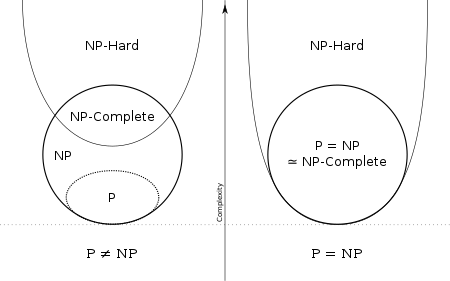
\includegraphics[width=60mm]{P_np.svg}
	\end{center}
	\caption{P, NP, NP-complete \& NP-hard sets \cite{P_NP_Figure}}
\end{figure}

\textbf{How to prove NP completeness generally?}
Call the problem we wish to prove is NP-complete $x$. First show there exists a verifier for $x$ with a polynomial or less
runtime, this is a algorithm that decides if a proposed solution to problem $x$ is correct. Then take a known NP-complete
problem call this $y$, and reduce it to $x$, one does this by transforming the input of $y$ to the input of $x$ in polynomial
time, we call this function $g(y)=x$. Assume there exists a polynomial time algorithm to solve $x$, $f()$ we could solve $y$ in
polynomial time too, $f(g(y))$, this implies P=NP, a contradiction. Therefore a polynomial time algorithm does not exist for
$x$.

\textbf{Our base NP-complete problem.} If, as the above suggests, we require a NP-complete problem to prove a problem is
NP-complete then we seem to have reached a paradox. Luckily we have the Cook-Levin Theorem.

\textit{Cook-Levin Theorem:} SAT is NP-Complete \textit{CITE }

\textbf{Def$^n$}: SAT is the following decision problem. Given a set of boolean variables $B$ and a collection of clauses $C$
does a valid truth assignment exist that satisfies $C$?

We now have a NP-complete problem to reduce other problems to.

\textbf{Let's make this more intuitive with examples.} 

\section{Verification is Easy}
Verificaiton decision problem, "is the sudoku puzzle complete?":

		\begin{equation}
			\Psi(S(,)) = \begin{cases}	
				\text{True if the puzzle is complete} \\
				\text{False if the puzzle is not complete}.
			\end{cases}
		\end{equation}

There exists an algorithm to do this in polynomial time with respect to the dimensions of the grid. 
\begin{enumerate}
\item For each row in the grid check there exists no repeated numbers. $O(n^2)$
\item For each column in the grid check there exists no repeated numbers. $O(n^2)$
\item For each box in the grid check there exists no repeated numbers. $O(n^2)$
\end{enumerate}
If all tests pass return True else return False.
This algorithm has complexity of $O(n^2 + n^2 + n^2) = O(3n^2) = O(n^2)$, this is polynomial and therefore $\Psi(S(,)) \in P$.


%%%%%%%%%%%%%%%%%%%%%


	\section{Existance is Hard}
		
Checking if a solution to sudoku exists is NP-complete, let us define the decision problem:

		\begin{equation}
		        \Phi (S(,)) = \begin{cases}
		            \text{True if a completion exists} \\
		            \text{False if a completion does not exist}.
				\end{cases}
		\end{equation}

Our question is does there exist a function $\Phi$ that when given an instance of the problem will, in polynomial time or less,
return True if it can be solved and False otherwise.

\subsection{Proof Outline}

The verifier is $O(n^2)$, as will be seen in the above subsection 'Validation is Easy', this shows the Sudoku decision problem
belongs to the set NP.

Now we need a reduction from sudoku to a known NP-complete problem to prove sudoku is also NP-hard. We will be creating a chain
of reductions: \textbf{Sudoku $\geq_p$ Latin Square $\geq_p$ Triangulated Tripartite $\geq_p$ 3SAT $\geq_p$ SAT}.

As the Sudoku decision problem is a member of NP and NP-hard it is NP-complete by definition.

\textbf{Note}: Theoretically any problem in the set NP-complete can be reduced to Sudoku and therefore this reduction is not
unique, however, it is the most intuitive way. Some readers may question why we are not looking at a reduction to a Graph
$n^2$-Colouring problem but in section \textbf{cite} we explore this is the wrong direction of reduction.

%%%%%%%%%%%%%%%%%%%%%%%


\subsection{Sudoku $\geq_p$ Latin Square}

\textbf{Def$^n$}: A valid Latin Square puzzle is a function $L:i,j \rightarrow x$ for values $i,j \in \{1,..,D\} $ and $x \in
\{0,...,D\}$ satisfying the following:
\begin{itemize}
\item{for all $a,b,c \in \{1,...,D\}$ with $L(a,b) \neq 0 $ and $L(a,c) \neq 0$ then $L(a,b) \neq L(a,c)$}
\item{for all $a,b,c \in \{1,...,D\}$ with $L(a,b) \neq 0 $ and $L(c,b) \neq 0$ then $L(a,b) \neq L(c,b)$}
\end{itemize}
It is complete or solved if for all $i,j \in \{1,...,D\}$, $L(i,j) \neq 0$.

By observation we see this is a superset of the sudoku puzzle, we just add the restrictions that the dimension must be a square
number and also add the third property of the sudoku puzzle defintion.

\textit{What is the Latin Square decision problem?} Given a latin square puzzle $L(,)$, can the function be augmented, by
changing only the value of the function for value pairs $i,j$ that previously gave $L(i,j) =0$, to get a complete latin square
puzzle?


\textit{Proof idea:} We must reduce a given latin square grid of size $D \times D$ to a sudoku grid size $D^2 \times D^2$ that
is solvable iff the Latin square is.

\textbf{Lemma:} Let $S_l$ be a Sudoku problem with the following construction 
\begin{equation}
	S_l(i,j) =\begin{cases}
0 \qquad\qquad\qquad\qquad\qquad\qquad\text{when } (i,j) \in L_s \\ 
((i-1 \text{ mod } n)n + \left\lfloor{i-1/n}\right\rfloor+j-1)\text{ mod } n^2 +1 \quad\text{otherwise}
\end{cases}
\end{equation}
where $L_s=\{(i,j)| \left\lfloor{i-1/n}\right\rfloor=0 \text{ and }(j \text{ mod }n)=1\}$. Then there exists an augmentation
$S_l'$ to complete the sudoku puzzle if and only if the square $L$ such that $L(i,j/n)=S_l'(i,j)-1/n+1$ for all $(i,j) \in L_s$
is a Latin square.

\textbf{Note:} The fact we have a formula to generate a valid sudoku for any size $D^2$ is interesting and we should explore if
this can be done for a $M\times N$ sudoku too. (explored in section 3).
Figure \ref{formula} gives examples of generated sudokus from this formula.

\begin{figure}[h]
\centering
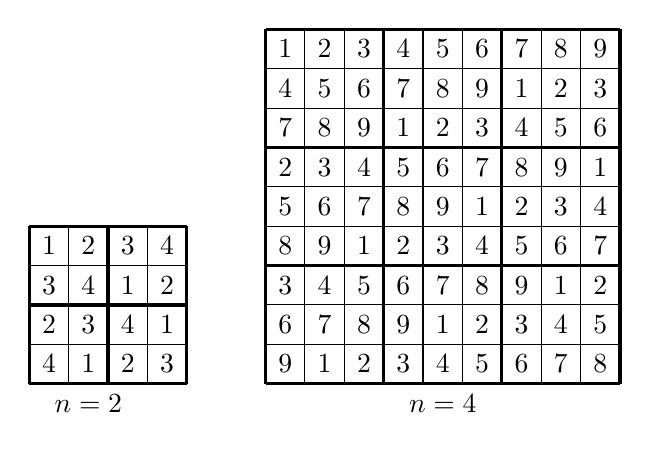
\begin{tikzpicture}[scale=.5]
\begin{scope}[xshift=10cm]
    \draw (0, 0) grid (4, 4);
    \draw[very thick, scale=2] (0, 0) grid (2, 2);
    \setcounter{rowa}{1}
    \setrowa {1}{2}{3}{4}
    \setrowa {3}{4}{1}{2}
    \setrowa {2}{3}{4}{1}
    \setrowa {4}{1}{2}{3} 
    \node[anchor=center] at (1.5, -0.5) {$n=2$};
  \end{scope}
  \begin{scope}[xshift=16cm]
    \draw (0, 0) grid (9, 9);
    \draw[very thick, scale=3] (0, 0) grid (3, 3);
    \setcounter{row}{1}
    \setrow {1}{2}{3}  {4}{5}{6}  {7}{8}{9}
    \setrow {4}{5}{6}  {7}{8}{9}  {1}{2}{3}
    \setrow {7}{8}{9}  {1}{2}{3}  {4}{5}{6}
    \setrow {2}{3}{4}  {5}{6}{7}  {8}{9}{1}
    \setrow {5}{6}{7}  {8}{9}{1}  {2}{3}{4}
    \setrow {8}{9}{1}  {2}{3}{4}  {5}{6}{7}
    \setrow {3}{4}{5}  {6}{7}{8}  {9}{1}{2}
    \setrow {6}{7}{8}  {9}{1}{2}  {3}{4}{5}
    \setrow {9}{1}{2}  {3}{4}{5}  {6}{7}{8}
    \node[anchor=center] at (4.5, -0.5) {$n=4$};
  \end{scope}
\end{tikzpicture}
\caption{Formula Generation of Valid Sudoku}
\label{formula}
\end{figure}

\textit{Proof:}

First we must show $S_l(i,j)=((i-1 \text{ mod } n)n + \left\lfloor{i-1/n}\right\rfloor+j-1)\text{ mod } n^2 +1$ forms a
complete and valid sudoku puzzle.

When $i=[1,...,n^2]$ then:
\begin{align}
	0&<\left\lfloor{i-1/n}\right\rfloor<n-1\\
	0&<i-1 \text{ mod } n<n-1\\
	0&<(i-1 \text{ mod } n)n + \left\lfloor{i-1/n}\right\rfloor<n^2-n\\
	0&<(i-1 \text{ mod } n)n + \left\lfloor{i-1/n}\right\rfloor+j-1<n^2-1\\
	1&<((i-1 \text{ mod } n)n + \left\lfloor{i-1/n}\right\rfloor+j-1)\text{ mod } n^2 +1<n^2\\
	1&<S_l(i,j)<n^2
\end{align} 
Note $\left\lfloor{i-1/n}\right\rfloor$ gives the row coordinate when indexed at 0 in which the larger box that (i,j) belongs
to starts and $i-1 \text{ mod } n$ gives the row within that box when indexed at 0. Therefore
$(\left\lfloor{i-1/n}\right\rfloor,i-1 \text{ mod } n)$ will take all value pairs of integers between 0 and $n-1$.

When j is fixed (particular column), assume two cells have the same value, that is $S_l(i,j)=S_l(i',j)$ then
\begin{align}
(i-1 \text{ mod } n)n + \left\lfloor{i-1/n}\right\rfloor+j-1 &= (i'-1 \text{ mod } n)n +
\left\lfloor{i'-1/n}\right\rfloor+j-1\\
	(i-1 \text{ mod } n)n + \left\lfloor{i-1/n}\right\rfloor &= (i'-1 \text{ mod } n)n + \left\lfloor{i'-1/n}\right\rfloor
\end{align}
from the above $i=i'$. No cell on a column has the same value.

When i is fixed (particular column) assume two cells have the same value, that is $S_l(i,j)=S_l(i,j')$ implies $j-1=j'-1 (mod
n)$ therefore $j=j'$.

For the third condition fix $\left\lfloor{i-1/n}\right\rfloor$. (i-1 \text{ mod } n,j) takes all value pairs of integers 0 to
n-1 so if a cell has the same value as another within the n by n square $S_l(i,j)=S_l(i',j')$ implying $(i-1 \text{ mod }
n,j)=(i'-1 \text{ mod } n,j')$ which means $i=i'$ and $j=j'$. Therefore $S_l$ is a valid and complete sudoku puzzle.

Now consider which integers fill the blanks in $L_s$. For $(i,j)\in L_s$, $S_l(i,j)-1= ((i-1 \text{ mod } n)n+j-1)\text{ mod }
n^2$ as $j mod n=1$, $j-1modn=0$ therfore $S_l(i,j)-1$ is divisible by n so $S_l-1/n+1$ gives integers between $[1,...,n]$.
Therefore $L(i,j) \in [0,...,n]$.

We must validate the Latin square conditions. The row constraint in $S_l$ ensures $S'(i,j)=S'(i,j') \implies j=j'$,
$S'(i,j)-1/n+1=S'(i,j')-1/n+1 \implies j=j'$, $L(i,j/n)=S'(i,j'/n) \implies j=j'$ is equivalent to the row constraint of L. The
column constraint of $S_l$ is equivalent to the column constraint of L. The small square constraint of $S_l$ is equivalent to
the column constraint of L. $\square$


%%%%%%%%%%%%%%%%%%%%%%%%%%%%%%%


\subsection{Latin Square $\geq_p$ Triangulate A Tripartite Graph}

\textbf{Def$^n$}: A graph $G=(V,E)$ is tripartite if a partition $V_1$, $V_2$, $V_3$ exists such that the vertices are split
into three sets with no edges between vertices that belong to the same set, i.e for all $(v_i,v_j) \in E\text{ if } v_i \in
V_i\text{ then }v_j \not\in V_i $.

\textbf{Def$^n$:} A triangulation T of a graph is a way to divide edges into disjoint subsets $T_i$, each forming a triangle
($T_i=\{(v_{1}, v_{2}),(v_{2}, v_{3}),(v_{3},v_{1})\}$).

If a tripartite graph can be triangulated it must be uniform, that is: every vertex in $V_1$ (or $V_2$ or $V_3$) has the same
number of neighbour in $V_2$ and $V_3$ (or the respective sets).

\textit{What is the Triangulated Tripartite decision problem?} Given a graph G that is tripartite (can be split into 3
subgroup, within these subgroups vertices should not share edges) can it be triangulated ?

\textbf{Theorem:} Completing a Latin square with dimensions n by n is equivalent to triangulating a tripartite graph $G= V_1,
V_2, V_3$.

\textit{Proof:} 

Intuitively, we map a graph to a Latin square $L$ through the following: 
given tripartite graph G=(V,E) label vertices in $V_1$ with distinct lables $\{r_1,...r_n\}$, label vertices in $V_2$ with
distinct lables $\{c_1,...c_n\}$ and label vertices in $V_3$ with distinct lables $\{e_1,...e_n\}$. Add edges such that:
\begin{itemize}
\item{If $L(i,j) = 0$ then add the edge $(r_i,c_j)$ }
\item{If for all $i \in [0,...,n]$ and constant j, $L(i,j) \neq k$ then add the edge $(r_i,e_k)$}
\item{If for all $j \in [0,...,n]$ and constant i, $L(i,j) \neq k$ then add the edge $(c_j,e_k)$}
\end{itemize}
This graph has a triangulation iff $L(i,j)$ can be solved.

\textbf{EXAMPLE}

Let us show every uniform tripartite graph can be transformed to the above formulation of a Latin square.

First we need an intermediate that is a generalisation of a latin square

\textbf{Def$^n$}: A Latin framework LF for tripartite graph G, size (r,s,t) is a r by s array with values [1,...,t]. With
constraints:
\begin{itemize}
\item{Each row/column contain each element only once.}
\item{If $(r_i,c_j)\in E$ then LF(i,j)=0 else LF(i,j)= k, $k\in [1,...,t]$}
\item{If $(r_i,e_k)\in E$  then $\forall j$ $LF(i,j)\neq k$}
\item{If $(c_j,e_k)\in E$  then $\forall i$ $LF(i,j)\neq k$}
\end{itemize}
If r=s=t then LF is a latin square (formulation above) which can be completed iff G has a triangle partition.

\textbf{Lemma}: For tripartite graph G=(V,E) with $|V_1|=|V_2|=|V_3|=n$ (uniform), there's a Latin framework of (n,n,2n).

\textit{Define LF an n by n array. For $(r_i,c_j)\in E$ $LF(i,j)=0$ else $LF(i,j)=1+n+((i+j)mod n)$. LF is a latin framework as
the first two bullet points of the definition hold by construction and as $1+n\leq LF(i,j)\leq 2n$ LF will never equal a value
in $1,...n$ and therefore the last two bullet points hold. The size is trivial. $\square$}

\textbf{Lemma}: Given latin framework LF(n,n,2n) for uniform tripartite graph G, we can extend the latin framework to have size
(n,2n,2n).

\textit{First we have a few denotions: R(k) = the number of times k appears in L plus half $|e_k|$; $S_i=\{k|k \not\in LF(i,j)
\forall j \cap (r_i,e_k)\not\in E\}$; $M=\{k|R(k)=r+s-t\}$.}
We show sets $S_1,...S_r$ have a system distinct representative (\textbf{DEFINE}) containing all elements of $M$, we then add
this system as the $(s+1)$st column and repeat until we have $2n$ columns.

Using Hoffman and Kuhn's theorem \textbf{CITE} we need only show that $S_1,...S_r$ have a system distinct representative and
that for every $M'\subseteq M$ at least $|M'|$ of sets $S_1,...S_r$ have non empty subsections with $M'$.

First choose any $m$ sets such that $1\leq m \leq r$. As G is uniform each set has t-s elements, so $m$ sets together have
$m(t-s)$ cardinality.Each value $1,...,t$ appears at least r+s-t times in $LF$, so note each value appears in at most $t-s$ of the sets $S_i$. Consider the union of the $m$ sets, this contains some $p$ elements so we have $p(t-s)\geq m(t-s)$ therfore $p\geq m$. So any $m$ sets have at least $m$ elements in their union and by the P Hall theorem \textbf{CITE} a system distinct representative exists.

Next take $M'\subseteq M$ and assume there are $p$ sets in $S_1,...S_r$ that have a nonempty intersection with $M'$. Each set has $t-s$ elements and together have caridinality $p(t-s)$, each element of $M$ appears in exactly $r-(r+s-t)=t-s$ of the $s_i$s, therefore $|M'|(t-s)\leq p(t-s)$ so $|M'|\leq p$. At least $|M'|$ sets have nonempty intersections with $M'$.

The Hoffman and Kuhn theorem holds and therefore a system distinct representative exists and can be added to the end. We repeat this n times. $\square$

\textbf{Lemma}: Latin framework (n,2n,2n) for grpah G, can be extended to (2n,2n,2n).

\textit{We can transpose the array and do the same as the previous lemma. $\square$}

\textbf{Note}: we can find a system distinct representative using the Hopcroft-Karp \textbf{CITE} algorithm which solves bipartite matching in polynomial time. 

Given a tripartite graph G, if it is not uniform then no triangulation exists, else we apply above to produce a latin framework
of size (2n,2n,2n) in polynomial time. This is a Latin square which can be completed iff G has a triangulation. The latin
square problem has been reduced to the triangulating a tripartite graph problem. $\square$


%%%%%%%%%%%%%%%%%%%%%%%%%%%%%%%%


\subsection{Triangulated Tripartite $\geq_p$ 3SAT}

\textit{What is 3SAT?} With a set of boolean variables $B$ and a collection of clauses $C$, with at most 3 literals (a literal
is any $b \in B$ or its negation $\bar{b}$) in each, does a valid truth assignment exist that satisfies $C$?
		\begin{equation}
		        \phi (C,B) = \begin{cases}
		            \text{True if a truth assignment exists} \\
		            \text{False if a truth assignment does not exist}.
				\end{cases}
		\end{equation}
This decision problem is therefore an enforced limitation of SAT as defined in the section Computational Complexity.

\textit{Proof:}

This reduction is a little trickier as we need to introduce the Holyer graph $H$.

\textbf{Def$^n$}: The Holyer graph $H_{3,p}$ is the set of vertices $V=\{(x_1,x_2,x_3)\in \mathbb{Z}_p^3 \| x_1+x_2+x_3 \equiv 0 (mod p)\}$ and an edge exists between vertices $(x_1,x_2,x_3)$ and $(y_1,y_2,y_3)$ if distinct i,j and k exist such that:
\begin{itemize}
\item $x_i\equiv y_i (\text{mod }p)$
\item $x_j\equiv y_j+1 (\text{mod }p)$
\item $x_k\equiv y_k-1 (\text{mod }p)$
\end{itemize}
This is much easier to grasp with a diagram see figure \textbf{FIGURE}.
This graph is tripartite if and only if $p\equiv 0 $ (mod 3), this is demonstrated by a 3-colouring (a graph is tripartite if and only if it is 3-colourable) in figure \textbf{FIGURE}.

\textbf{Def$^n$}: $H_{3,p}$ has only two triangulations, termed a true and a false triangulation \textbf{FIGURE}. 

\textbf{Note:} We connect graphs together by taking a set of vertices in $G_1$ and making them the 'same' as a set of vertices in $G_2$, sets are the same size.

\textbf{Def$^n$}: We will connect out graph with F-patches and T-patches \textbf{FIGURE}. 

\textbf{Lemma}: Connecting two $H_{3,p}$ by two A-patches then our triangulations of these graphs can be of the form $(T,T)$, $(T,F)$ or $(F,T)$. Then by removing the centre triangles from both graphs we get only the triangulations $(T,F)$ or $(F,T)$. If we expand this to $x$ $H_{3,p}$ we get only one false triangulation and the rest true.

Transformation process: (select p large enough to prevent patch overlap and  $p\equiv 0 $ (mod 3))
\begin{itemize}
\item For $b_i\in B$ create $H_{3,p}$ called $G_{b_i}$.
\item For all $c_j\in C$, for each literal $l_{i,j}$ $j\in [1,2,3]$ create $H_{3,p}$ called $G_{i,j}$.
\item If $l_{i,j}=b_k$ connect an F-patch in $G_{b_k}$ to an F-patch in $G_{i,j}$, else if $l_{i,j}=\neg b_i$ connect a F-patch in $G_{i,j}$ to a T-patch in $G_{b_k}$.
\item For each $i$ connect one F-patch from each $G_{i,1}$, $G_{i,2}$ and $G_{i,3}$ then delete the centre triangle. 
\item $G = \{G_{b_i}$ $|$ $b_i \in B\}\cup\{G_{i,j}$ $|$ $ c_j\in C\text{ and }i\in [1,..,3] \}$
\end{itemize}

We now need to prove the graph produced by the above transformation can be triangulated if and only if there is a truth assignment satisfying the 3SAT formula.

 Assume a triangulation of G exists, consider a H within the construction of G. H is eitehr a true triangulation or a false triangulation. Now assume $l_{i,j}$ is $b_k$ and consider the join between $G_{i,j}$ and $G_{b_k}$ as this joins two F-patches we get at least one true triangulation. (if $G_{i,j}$ is a true triangulation this acounts for all edges near the joining patch but the actual patch can be attributed to $G_{b_k}$ which can be triangulated either way, if both are false triangulations the connecting patch is forced to belong to both $G_{i,j}$ and $G_{b_k}$ which is a contradiction.)

Similarly if  $l_{i,j}=\neg b_i$ then $G_{i,j}$ is a false triangulatio or $G_{b_k}$ is a true triangulation.

Next the join between clause graphs allow for one false triangulation and the rest  are true triangulations. As the centre of the patch is missing a single $G_{i,j}$ must take the outer edges of the patch by being a false triangulation.

If G can be triangulated a truth assignment exists such that variable $b_k$ is true if $G_{b_k}$ has a true partition otherwise it is false.

If there exists a truth assignment we can triangulate $G_{b_k}$ according to this truth assignment and this will allow for the whole graph to be triangulated.

This transformation takes place in polynomial time and therefore Triangulated Tripartite $\geq_p$ 3SAT. $\square$

%%%%%%%%%%%%%%%%%%%%%%%%%%%%%%%%

\subsection{3SAT is NP-Complete}
%%%%% define clause

\textit{Proof:}

Given a truth assignment $t$ check each clause is satisfied, if all are satisfied return True else False, this algorithm is at
most the length of $C$ multiplied by the length of $B$. $O(BC)$ is polynomial, a polynomial verifier exists.

Given a SAT instance with the input sets of $B$ and $C$. $C$ is in conjunctive normal form (every clause set can be converted
to an equivalent set in CNF form \cite{CNF}) such that $\forall c \in C$ and for some $b_1, ... ,b_n \in B$, $c = b_1 \lor b_2
\lor ... \lor b_n$. For each $c \in C$ with more than 3 literals we can transform these to a new set of clauses of length 3.

For $c = b_1 \lor b_2 \lor ... \lor b_n$ we introduce a new literal: $a_1$ to give $b_1 \lor b_2 \lor a_1$, $\bar{b_1} \lor
a_1$, $\bar{b_2} \lor a_1$ and $a_1 \lor b_3 \lor ... \lor b_n$. Then $a_1 \lor b_3 \lor ... \lor b_n$ becomes $b_3 \lor b_4
\lor a_2$, $\bar{b_3} \lor a_2$, $\bar{b_4} \lor a_2$ and $a_1 \lor a_2 \lor b_5 \lor ... \lor b_n$. This continues at most
$n/2$ times to give $a_1 \lor ... \lor a_{n/2}$ or $a_1 \lor ... \lor a_{n/2} \lor b_n$ if n is odd.

Because we can convert a clause larger than 3 into multiple clauses of at most 3 literals in linear time ($O(n/2 + n/4 + ...) =
O(n)$) this means we can reduce SAT to 3SAT in polynomial time.

As SAT is NP-complete by the Cook-Levin Theorem, this proves 3SAT is NP-Complete. $\square$
		
\begin{figure}
\begin{center}
		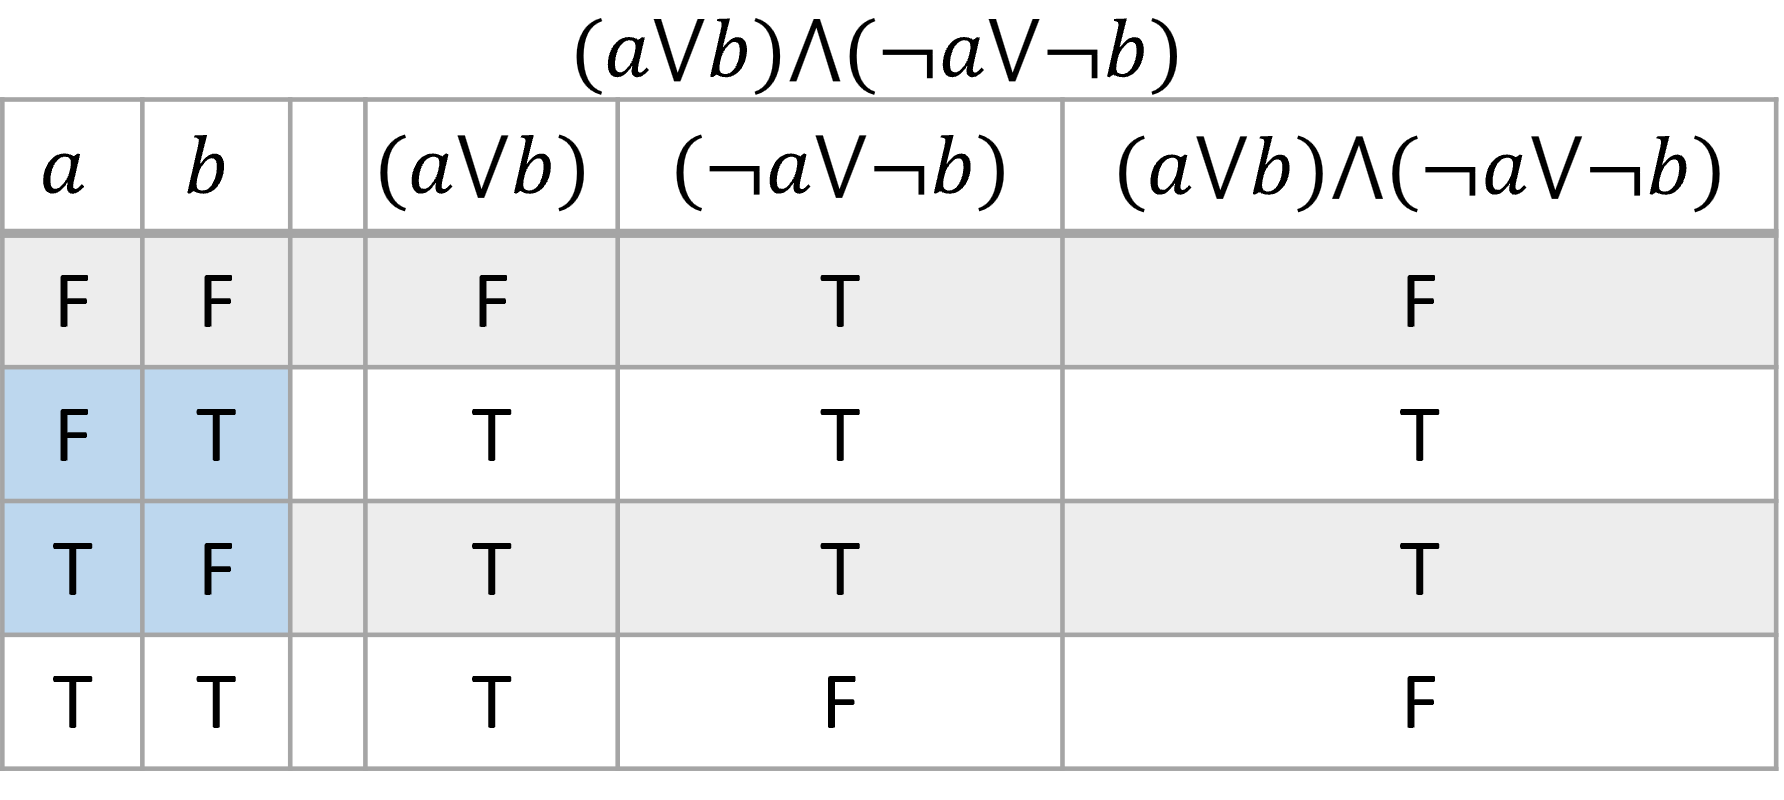
\includegraphics[width=70mm]{figures/sat_example.png}
\end{center}
		\caption{Truth Assignment Example with Highlighted Valid Assignment}
\end{figure}

%%%%%%%%%%%%%%%%%%%%%%%%%%%%%%%%

\subsection{Sudoku $\geq_p$  Graph Colouring}

%%%%%%%%%%%%%%%%%%%%%%%%%%%%%%%%

\subsection{Example, dimension analysis}

%%%%%%%%%%%%%%%%%%%%%%%%%%%%%%%%

\section{Determining Uniqueness is Hard}

\textbf{Def$^n$:} The Sudoku Uniqueness problem is: Given a partially completed sudoku grid $S$ does only a single completion
exist?
		\begin{equation}
		        \Gamma (S) = \begin{cases}
		            \text{True if only a single completion exists} \\
		            \text{False if multiple completions or none exist}.
				\end{cases}
		\end{equation}

This is NP-hard (no polynomial verifier exists), NP-complete reduction exists.

It is hard to determine if a puzzle has a unique solution. 	 \textit{TO COMPLETE: FIND PAPER WITH PROOF}
		
% ~~~~~~~~~~~~~~~~~~~~~~~~~~~~~~~~~~~~~~~~~~~~~~~~~~~~~~~~~~~~~~~~~~~~~~~~~~~~~~~~~~~~~~~~~~~~ %
\chapter{Solving Techniques}
\section{Backtracking}
The standard way to solve a $9 \times 9$ sudoku puzzle is by the backtracking algorithm. This is a brute force method with a
few optimisations. One can expect to find this algorithm in a computer science course introduction to recursion, that is to say
it is not a complex concept and while useful for the usual sizes, as soon as we increase to $16 \times 16$ this becomes
infeesible.

\begin{algorithm}
\caption{Backtracking}
\begin{algorithmic}
\Procedure{ Backtracking}{grid}
    \For {row}
        \For {column}
            \If{grid(row,column) = 0}
                \State{try a value in this position}
                \State{Backtracking(grid with new value)}
                \If{successful}
                    \State{return grid}
                \Else:
                    \State{try another value}
	       \EndIf
                \If{no values left to try}
                    \State{return False}
		\EndIf
\EndIf
\EndFor
\EndFor
    \State{return grid}
\EndProcedure						
\end{algorithmic}
\end{algorithm}
Why does brute force not work for larger examples? It will work \textit{TO DO: PROVE ALG CORRECTNESS} but due to the complexity
of the problem (point back to sudoku is hard chapter) it is infeesible.
\section{Simulated Annealing} 

Based on metalurgy

\begin{algorithm}
\caption{Simulated Annealing}
\begin{algorithmic}
\Procedure{SimAnnealing}{grid, schedule, f}
	\State{current = initialise state}
	\For {$t=1 \text{to} \inf$ }
		\State{T=schedule[t]}
		\If{$T\leq  \epsilon$}
			\State{return current}
		\Else
			\State{choose successor at random}
			\State{$\Delta E$ = f(successor) - f(current)}
			\If{$\Delta E \geq 0$}
				\State{current = succ}
			\Else{ choose with probability $e^{\frac{\Delta E}{T}}$}
				\State{current = successor}
			\EndIf
		\EndIf
	\EndFor
\EndProcedure
\end{algorithmic}
\end{algorithm}

\subsection{Convergence}
\subsection{Speed of Convergence}
\cite{simulated annealing} one of 100 most cited papers, one of the first AI algs

% ~~~~~~~~~~~~~~~~~~~~~~~~~~~~~~~~~~~~~~~~~~~~~~~~~~~~~~~~~~~~~~~~~~~~~~~~~~~~~~~~~~~~~~~~~~~~ %
\chapter{Group theory}
\section{Starting Simple $4 \times 4$}
Let us analyse Shidoku which is a specific set of sudokus with dimensions 4 by 4 the smallest non trivial sudoku puzzle. Only 2
fundamentally different. One has 96 identical, other has 192. Why not the same amount?



	\section{Equivalence Classes}
	\section{$6 \times 6$}

Define Rodoku 
Define which sudoku sizes can exist


812
	\section{$8 \times 8$}
	\section{$9 \times  9$}
5,472,730,538
% ~~~~~~~~~~~~~~~~~~~~~~~~~~~~~~~~~~~~~~~~~~~~~~~~~~~~~~~~~~~~~~~~~~~~~~~~~~~~~~~~~~~~~~~~~~~~ %
\chapter{Other}
% ~~~~~~~~~~~~~~~~~~~~~~~~~~~~~~~~~~~~~~~~~~~~~~~~~~~~~~~~~~~~~~~~~~~~~~~~~~~~~~~~~~~~~~~~~~~~ %
\section{Other Related Problems}
	\subsection{Latin Squares}

		\begin{itemize}
		\item{A latin square is an n by n matrix filled with n characters that must not repeat along columns or rows.}
		\item{Reduced Form - f first row and column is in the natural order}
		\item{Equivalence classes}
		\item{Number of n by n latin squares is bounded}
		\item{Latin squares can be considered a bipartite graph}
		\item{Agronomic Research}
		\item{Latin hypercube}
		\end{itemize}

	\section{Magic Squares}

		\begin{itemize}
		\item{A magic square is a matrix of numbers with each column, row and diagonal summing to the same value, 
		this value is known as a magic constant and the degree is the number of columns/rows.}
		\item{A normal magic square is one containing the integers 1 to $n^2$.}
		\item{Magic Squares with repeating digits are considered trivial.}
		\item{Semimagic squares omit the diagnonal sums also summing to the magic constant.}
		\item{Truly thought to be magic Shams Al-ma'arif.}
		\item{Generation, there exists not completely general techniques. Diamond Method}
		\item{Associative Magic Squares}
		\item{Pandiagonal Magic Squares}
		\item{Most-Perfect Magic Squares}
		\item{Equivalence classes for $n<=5$ but not for higher orders.}
		\item{The enumeration of most perfect magic squares of any order.}
		\item{880 distinct magic squares of order four}
		\item{Normal magic squares can be constructed for all values except 2}
		\item{Preserving the magic property when transformed}
		\item{Methods of construction}
		\item{Multiplicative magic squares - produce infinite}
		\item{Sator square}
		\item{magic square of squares - Parker Square is a failed example of this}
		\end{itemize}
	
	\subsection{Greco-Latin Squares}

		\begin{itemize}
		\item{Two orthogonal latin squares super imposed, such that the pairs of values are unique.}
		\item{Group based greco latin squares}
		\item{Eulers interest came from construction of magic squares}
		\item{Exists for all but 2 and 6.}
		\end{itemize}
% ~~~~~~~~~~~~~~~~~~~~~~~~~~~~~~~~~~~~~~~~~~~~~~~~~~~~~~~~~~~~~~~~~~~~~~~~~~~~~~~~~~~~~~~~~~~~ %

\section{Generating  Techniques}
A polynomial generation algorithm without requiring a uniqueness checker which we have proven to be np-complete and therefore
infeesible for large n.
~~~~~~~~~~~~~~~~~~~~~~~~~~~~~~~~~~~~~~~~~~~~~~~~~~~~~~~~~~~~~~~~~~~~~~~~~~~~~~ %
\section{17 is the Magic Number}
	4 for shidoku
	\subsection{Sparsity - information theory}
		Bomb sudoku/latin squares - Additional rule: the same number can not occur in adjacent or diagonally adjacent squares.
% ~~~~~~~~~~~~~~~~~~~~~~~~~~~~~~~~~~~~~~~~~~~~~~~~~~~~~~~~~~~~~~~~~~~~~~~~~~~~~~~~~~~~~~~~~~~~ %

\section{Topology}
	\subsection{Torus}
% ~~~~~~~~~~~~~~~~~~~~~~~~~~~~~~~~~~~~~~~~~~~~~~~~~~~~~~~~~~~~~~~~~~~~~~~~~~~~~~~~~~~~~~~~~~~~ %
\section{Polynomials \& Constraint Programming}
	Use of polynomials
	Roots of unity
	Grobner Basis
% ~~~~~~~~~~~~~~~~~~~~~~~~~~~~~~~~~~~~~~~~~~~~~~~~~~~~~~~~~~~~~~~~~~~~~~~~~~~~~~~~~~~~~~~~~~~~ %
\begin{thebibliography}{100}
	\bibitem{P_NP_Figure} https://en.wikipedia.org/wiki/NP\_(complexity)
\bibitem{CNF} Artificial Intelligence: A modern Approach Archived 2017-08-31 at the Wayback Machine [1995...] Russell and
Norvig
\bibitem{GeneratingAlg}
https://www.researchgate.net/publication/251863893\_A\_New\_Algorithm\_for\_Generating\_Unique-Solution\_Sudoku
	\bibitem{Complexity} https://fse.studenttheses.ub.rug.nl/22745/1/bMATH\_2020\_HoexumES.pdf.pdf
\bibitem{latin to tripartite} http://web.math.ucsb.edu/\~padraic/mathcamp\_2014/np\_and\_ls/mc2014\_np\_and\_ls\_lecture3.pdf,
http://web.math.ucsb.edu/\~padraic/mathcamp\_2014/np\_and\_ls/mc2014\_np\_and\_ls\_lecture4.pdf
	\bibitem{tripartite to sat} https://scholar.rose-hulman.edu/cgi/viewcontent.cgi?article=1398\&context=rhumj
	\bibitem{LatinSquaresAlgorithm} https://onlinelibrary.wiley.com/doi/10.1002/(SICI)1520-6610(1996)4:6<405::AID-JCD3>3.0.CO;2-J
	\bibitem{LatinSquareAgronomicResearch} http://joas.agrif.bg.ac.rs/archive/article/59
\bibitem{LatinSquareCommunication}
https://www.semanticscholar.org/paper/Permutation-arrays-for-powerline-communication-and-Colbourn-Kløve/7e69cfdbd2082463c66de698da1e326f0556d1d4
	\bibitem{MagicSquares1} http://www.multimagie.com/English/SquaresOfSquaresSearch.htm
	\bibitem{MagicSquaresRelationToSudoku} https://plus.maths.org/content/anything-square-magic-squares-sudoku
	\bibitem{Programming Sudoku} https://link.springer.com/book/10.1007/978-1-4302-0138-0
\bibitem{simulatedannealing}an Laarhoven, P.J.M., Aarts, E.H.L. (1987). Simulated annealing. In: Simulated Annealing: Theory
and Applications. Mathematics and Its Applications, vol 37. Springer, Dordrecht. https://doi.org/10.1007/978-94-015-7744-1\_2
\end{thebibliography}
\end{document}
\vspace{5mm}